\documentclass[conference]{IEEEtran}
%\IEEEoverridecommandlockouts
% The preceding line is only needed to identify funding in the first footnote. If that is unneeded, please comment it out.
%\usepackage{cite}
\usepackage{amsmath,amssymb,amsfonts}
\usepackage{algorithmic}
\usepackage{graphicx}
\usepackage{textcomp}
\def\BibTeX{{\rm B\kern-.05em{\sc i\kern-.025em b}\kern-.08em
    T\kern-.1667em\lower.7ex\hbox{E}\kern-.125emX}}
\usepackage{mathtools}

\usepackage[backend=biber]{biblatex}
\addbibresource{references.bib}

\DeclareMathOperator*{\argmin}{argmin}
\DeclareMathOperator{\E}{\mathbb{E}}
\newcommand{\norm}[1]{\left\lVert#1\right\rVert}

\renewcommand*{\bibfont}{\footnotesize}

\begin{document}

\title{Optimal Control of Hybrid Energy Storages in Electric Vehicles}

\author{\IEEEauthorblockN{Alok Deshpande}
\IEEEauthorblockA{University of Toronto - Energy Systems}
}

%\newenvironment{psmallmatrix}
%  {\left[\begin{smallmatrix}}
%  {\end{smallmatrix}\right]}

\maketitle

%\begin{abstract}
%This document is a model and instructions for \LaTeX.
%This and the IEEEtran.cls file define the components of your paper [title, text, heads, etc.]. *CRITICAL: Do Not Use Symbols, Special Characters, Footnotes, 
%or Math in Paper Title or Abstract.
%\end{abstract}

\section{Introduction}
Battery life is a factor that is critical for electric vehicle (EV) operation. It impacts vehicle performance in that an aging battery experiences a drop in energy capacity \cite{shi2017optimal}, which reduces the maximum distance that can be travelled on a single charging. One promising way to prolong battery life is to use a hybrid energy storage system, composed of a combination of a battery and a secondary energy storage in parallel \cite{thounthong2009energy}, such as a supercapacitor \cite{bambang2014energy}\cite{thounthong2009energy}\cite{7939849}. 

Dynamic programming (DP) has previously been been applied in this context to determine an optimal sequence of controls -- that is to say, energy discharges from the battery and supercapacitor -- that satisfies a sequence of energy demands. \cite{su2013modeling} has employed DP with a black-box model of a single battery; we extend this to the two-storage case. Moreover, \cite{8330176} and \cite{8315074} have both solved the problem under the assumption of an infinite horizon, and we do so similarly.

However, our approach differs from these papers as we attempt to resolve the curse of dimensionality in the DP. We first reformulate the infinite horizon DP as a linear program (see, e.g., \cite{Bertsekas:2007:DPO:1396348}). We then construct an approximation using the technique given in \cite{deFarias:2003:LPA:970869.970918}. Finally, we generate basis functions for the approximation using the methods of \cite{Bellman:1957} and \cite{Bellman1962}. %\cite[pp. 323--324]{Bellman1962}.

We begin by modelling the problem in Section II and solving the exact equivalent problem in Section III. In Section IV, we explain how the basis functions are generated to approximate the solution to the exact LP, and hence we solve the approximate LP. Finally, in Section V, we show numerical results for the vehicle application and draw conclusions on the optimal response to various demand patterns. 

\section{Model}
In this section, we develop the model for the two storage device optimization problem. Just as in \cite{su2013modeling}, we assume that both time and state are discretized.

Firstly, let $E_{h})(t)$ and $D_{h}(t)$ denote the energy stored in and energy discharged from device $h$ at time instant $t$. Here $h=1$ refers to the battery and $h=2$ refers to the supercapacitor. As well, let $L(t)$ be the energy demand imposed on the system, and $C_{2}(t)$ be the energy input to the supercapacitor by charging. We now define the state to be $x(t):=(E_{1}(t),E_{2}(t),L(t))$ and the control to be $u(t):=(D_{1}(t),D_{2}(t))$. Note that $C_{2}(t)$ not part of the control because it is a dependent variable through the energy supply-demand balance, as explained below.

It is well established that the discrete-time state equation for the battery without regenerative braking is $f_{1}(\cdot)$, defined as follows:
\begin{math}E_{1}(t+1)=\beta_{1}E_{1}(t)-\frac{1}{\alpha_{1}^{D}}D_{1}(t)\end{math} Likewise, the state equation for the supercapacitor is $f_{2}(\cdot)$, defined as:
\begin{math}E_{2}(t+1)=\beta_{2}E_{2}(t)+\alpha_{2}^{C}C_{2}(t)-\frac{1}{\alpha_{2}^{D}}D_{2}(t)\end{math} Here, $\alpha^{C}_{h}$ and $\alpha^{D}_{h}$ respectively denote the charging and discharging efficiencies of device $h$, and $\beta_{h}$ is the storage efficiency factor for device $h$. The dynamics given by $f_{1}(\cdot)$ and $f_{2}(\cdot)$ can then be more generally represented by the function $f(x(t),u(t),w(t))$.

In this model, the energy in storage device $h$ is bounded in the range $E_{h}^{min}\leq E_{h}(t)\leq E_{h}^{max}$ where $E_{h}^{max}$ is the upper bound and $E_{h}^{min}$ is the lower bound, normally equal to zero. Likewise, the charging and discharging are bounded in the ranges $0\leq C_{h}(t)\leq C_{h}^{max}$ and $0\leq D_{h}(t)\leq D_{h}^{max}$, where $C_{h}^{max}$ and $D_{h}^{max}$ are the upper limits. Finally, energy supply-demand balance imposes the following constraint: $\left[D_{1}(t)\right] + \left[D_{2}(t) - C_{2}(t)\right] = L(t)$. These bounds serve as the constraints of the optimization problem.


There are two relevant costs in this model. The first is the cost of loss of energy due to transfers between the devices, which is $(1-\alpha_{1}^{D})D_{1}(t)+(1-\alpha_{2}^{C})C_{2}(t)+(1-\alpha_{2}^{D})D_{2}(t)$. We choose to weight the cost of the energy transfers by their inefficiencies ($1-\alpha$), as this penalizes the less efficient ones and the full objective is convex because it is constrained to be non-negative. The other cost is that for the discharge rate for the battery, simply given by $K\left[D_{1}(t)\right]^{2}$. Here $K$ is a weighting for this cost relative to the cost of energy loss. We choose this as the convex cost as it is referenced most commonly in literature \cite{bambang2014energy}, where it serves to penalize more for high excursions.

The sum of these objective functions is convex and constrained non-negative. Hence, the following optimization problem -- whose objective is this sum -- has a unique solution:

\begin{multline} \label{eq:initCostFnc}
    \min_{D_{1},D_{2},C_{2}}\Biggl[\sum_{t=0}^{T-1}
	(1-\alpha_{1}^{D})D_{1}(t)+
	(1-\alpha_{2}^{C})C_{2}(t)+\\
	(1-\alpha_{2}^{D})D_{2}(t)+
	K\left[D_{1}(t)\right]^{2}
	\Biggr]\end{multline}
subject to
\begin{displaymath}E_{h}^{min}\leq E_{h}(t)\leq E_{h}^{max}\end{displaymath}
\begin{displaymath}0\leq C_{h}(t)\leq C_{h}^{max}\end{displaymath}
\begin{displaymath}0\leq D_{h}(t)\leq D_{h}^{max}\end{displaymath}
\begin{displaymath}\left[D_{1}(t)\right] + \left[D_{2}(t) - C_{2}(t)\right] = L(t)\end{displaymath}
\begin{displaymath}E_{1}(t+1)=\beta_{1}E_{1}(t)-\frac{1}{\alpha_{1}^{D}}D_{1}(t)\end{displaymath}
\begin{displaymath}E_{2}(t+1)=\beta_{2}E_{2}(t)+\alpha_{2}^{C}C_{2}(t)-\frac{1}{\alpha_{2}^{D}}D_{2}(t)\end{displaymath}

Note that the energy balance equality constraint can be immediately substituted into the objective, which reduces the decision vector to $D:=(D_{1},D_{2})$. (More correctly, the minimization is done with respect to a vector $\textbf{D}$, whose components are $D(t)$ at $t=0,...,T-1$.  However, for the sake of clarity, we omit this formality.)

%Critically, this paper chooses to take the expectation after the minimization. This is done so that the net energy discharged (control, $D$) exactly matches the demand, $L$, at all times and not its expected value, ensuring supply-demand balance.

In this model, $L(t)$ is a time-varying quantity which is observed at time $t$ before the control $u(t)$ is applied, since the controller must have full knowledge of the demand before providing the control to satisfy it. Further, it evolves uncontrollably according to $L(t+1)=0L(t)+w(t)$, where $w(t)$ is a random variable which follows an unknown distribution and which represents a perturbation after the control is applied. %We have taken $L(t)$ to be part of the state. Doing so allows us to generate an optimal policy that a function of the load at time $t$, in addition to arbitrary energy state. (This choice of state makes the later LP formulation of this problem different from others reviewed in literature.)

The optimal value function \eqref{eq:initCostFnc} may be expressed in the general form:
\begin{equation}J^{*}[x(t)]=\min \Biggl\{\mathop{\E}_{w(t)}\left[\sum_{t=0}^{T-1}g(x(t),u(t),w(t))\right]\Biggr\}\end{equation}
where $g(\cdot)$ is called the stage cost. (Note that we avoid formality here, too, for brevity. Correctly, the expectation is with a respect to sequence of random variables whose terms are $w(t)$ at $t=0,...,T-1$.) The value function can then be re-written in the form of Bellman's equation, which allows the problem to be solved by dynamic programming:
\begin{displaymath}
J_{t}[x(t)]=\min g(x(t),u(t)) + \mathop{\E}_{w(t)} \{J_{t+1}[f(x(t),u(t),w(t))]\}
\end{displaymath}
starting from $J_{T}[x(T)]:=0$.

Note that in this model, the random perturbation $w(t)$ that determines $L(t+1)$ depends on the energy in the subsequent state, $E(t+1):=(E_{1}(t+1),E_{2}(t+1))$. This is because the demand at any iteration is limited to not exceed the total current energy at that iteration -- i.e. we assume that vehicle will not be completely depleted of fuel. However, the subsequent energy depends on the current energy through $f(\cdot)$, so in a manner respecting causality, the above expectation is more correctly conditioned on $x(t)$ and $u(t)$. While this conditioning is not shown, we do assume that the process generating $w(t)$ is Markovian.

%It is common knowledge that a finite number of iterations is sufficient to allow $J_{t}[x(t)]$ to reach a steady-state value of $J^{*}(x)$ within a tolerance $\epsilon$. The method of solving these multiple iterations is called discounted value iteration with bounded cost per stage. In Section V, we explain how we set this tolerance compared to that in the LP formulation. LP is now presented below.

%This DP program can be analyzed to determine its computational complexity. Firstly, with regards to the size of the problem, two matrices must hold data: the optimal cost, and the optimal control. By inspecting (6), it is clear that both the cost and control are functions of the state $(x,w)$, and so must have a size of $N\times M$. However, the previous costs must also be retained to determine that the costs are converging, so the required size is actually twice that (two matrices).

%The theoretical runtime can also be analyzed. Knowing that each iteration of DP involves nothing more than exhaustive searching (cost evaluation), and that $g(\cdot)$ is a function of the triplet $(x,u,w)$, the number of combinations to evaluate must be $NMP$. Over $k$ iterations, this is then $NMPk$ evaluations. According to theory \cite{Bertsekas:2007:DPO:1396348}, $k$ is related to the logarithm of the error tolerance on the constraints, and so it is also possible to estimate runtime in theory. However, this paper chooses to test the number of iterations from numerical examples, as detailed in Section 8.

%These computational characteristics for the DP will be compared to those of the LP, which is now presented below.


\section{Exact Solution of DP}
\subsection{Infinite Horizon DP}
The above problem can be solved for $T$ control periods. However, for the very large number of periods required in this application, the total value $J$ will approach infinity, since each stage cost is non-negative. Thus, it is necessary to discount future costs by a factor $0<\alpha<1$.

%With this modification, over multiple iterations the value function $J_{t}[x(t)]$ approaches the steady-state function $J(x)$. When a greedy policy is selected at each iteration, this function $J(x)$ is also optimal ($J^{*}(x)$). Hence, 
With this modification, the infinite horizon problem is:
\begin{multline} \label{eq:DP}
J^{*}(x)= \min\Biggl\{\mathop{\E}_{w(t)}\left[\sum_{t=0}^{\infty}\alpha^{t}g(x(t),u(t),w(t))\right]\Biggr\}
\end{multline}

When subject to the same constraints as \eqref{eq:initCostFnc}, this optimization problem is termed the infinite horizon DP formulation of optimal control for this paper. However, because we only use the infinite horizon approach for this application, henceforth we will simply use \textit{DP} to refer to this infinite horizon DP.

\subsection{Primal LP}
Given that the value $J_{t}[x(t)]$ approaches an upper bound of $J^{*}(x)$, as shown in \cite{Bertsekas:2007:DPO:1396348}, $J^{*}(x)$ can be calculated by solving an LP maximization problem. This LP has optimal \textit{solution} of $J^{*}(x)$, rather than its optimal value as in value iteration, so henceforth we use \textit{costs} of the LP to refer to the possible solutions and not values of the LP objective function.

In \cite{Bertsekas:2007:DPO:1396348}, Bertsekas presents an LP formulation of DP where the state has no uncontrollable components (in this case, the demand) that are randomly generated. We rewrite this in a form where the uncontrollable component is part of the state.

To this end, we firstly define three sets: $W$ as the set of random perturbations, indexed by $1\leq k \leq M$; $X$ as the set of states, indexed by $1\leq i \leq NM$; and $U$ as the set of controls, indexed by $1\leq p \leq P$. As well, let
$\lambda(x_{i})$ be the cost associated with state $x_{i}$ such that $\boldsymbol{\lambda(x)}$ is a vector with the elements being costs in each state. Let $g(x_{i},u_{p})$ be the stage cost, and let $p_{i,j}(u_{p})$ be the probability of moving from $x_{i}\in X$ to $x_{j}\in X$ by applying control $u_{p}\in U$. Note that the subscripts are indices for vectors in the sets. %, and not indices of iteration.

Then, the probability $p_{i,j}(u)$ is defined as: 
\begin{displaymath}
p_{i,j}(u_{p})= P(x_{j}| x_{i},u_{p})
\end{displaymath} For this probability to be non-zero, the next state $x_{j}$ must be a state $x_{i'}:=f(x_{i},u_{p},w_{k})$ that is accessible from the current state. In this case:
\begin{align*} 
p_{i,j}(u_{p})&= P(x_{i'}| x_{i},u_{p})\\ 
&= P(f(x_{i},u_{p},w_{k})| x_{i},u_{p})
\end{align*} The only random variable in the above expression is $w_{k}\in W$, so we may express this instead as a probability of $w_{k}$:
\begin{align*} 
    p_{i,j}(u_{p})&= P(w_{k} | x_{i},u_{p})
\end{align*}

Hence, with the uncontrollable component now being a part of the state, the LP in \cite{Bertsekas:2007:DPO:1396348} can be expressed as:

\begin{equation} \label{eq:prelimLP}
\min_{\lambda(x_{i}) \forall i} \sum_{i=1}^{NM} -\lambda(x_{i})
\end{equation}

subject to $\forall x_{i} \in X$: \begin{align*}
\lambda(x_{i})-\alpha\sum_{k=1}^{M}P(w_{k} | x_{i},u_{1})\lambda(f(x_{i},u_{1},w_{k})) &\leq g(x_{i},u_{1}) \\
&\vdots\\
\lambda(x_{i})-\alpha\sum_{k=1}^{M}P(w_{k} | x_{i},u_{P})\lambda(f(x_{i},u_{P},w_{k})) &\leq g(x_{i},u_{P})
\end{align*}

This is the LP to be solved to determine the solution to the DP. As a reminder, in the context of the hybrid storage problem, $x=(E_{1},E_{2},L)$ and $u=(D_{1},D_{2})$.

The problem can be expressed most succinctly in matrix form as:
\begin{equation} \label{eq:prelimLPmtx}
    \max_{\boldsymbol{\lambda_{p}}} \boldsymbol{1}^{T} \boldsymbol{\lambda_{p}}
    \hspace{1em}s.t.\hspace{1em}
    \boldsymbol{\lambda}-\alpha PF\boldsymbol{\lambda} \leq \boldsymbol{g}
\end{equation} Here, $\boldsymbol{\lambda} = [\boldsymbol{\lambda_{p}}\hdots \boldsymbol{\lambda_{p}}]^{T}$ is a vector containing P repeated vectors $\boldsymbol{\lambda_{p}}$. Each vector $\boldsymbol{\lambda_{p}}$ contains the current state costs, $\lambda(x_{i})$, as its components. Likewise, the vector $F\boldsymbol{\lambda}$ contains P repeated vectors each containing the costs for next states $x_{j}$, which are $\lambda(x_{j})$. And finally, vector $\boldsymbol{g}$ contains the stage cost for each state-control pair. 

In addition to this, $P$ is a transition probability matrix containing the conditional probabilities $p_{i,j}$. For the subset of its rows associated with the $p^{th}$ control -- i.e. the $p^{th}$ set of inequalities in \eqref{eq:prelimLPmtx} -- these probabilities are $p_{i,j}(u_{p})$. Hence, based on the prior definition of these elements $p_{i,j}(u_{p})$, one may note that its structure is:

\begin{displaymath}
p_{i,j}(u_{p}):=
\left\{
\begin{array}{l}
P(w_{k}|x_{i},u_{p}) \hspace{0.2cm} if \hspace{0.2cm} x_{j}=f(x_{i},u_{p},w_{k})\\
0 \hspace{1.8cm} otherwise
\end{array}
\right.
\end{displaymath}

%Firstly, one can consider just the subset of costs associated with the $p^{th}$ control. This is done because each of the sets of linear inequalities in \eqref{eq:prelimLP} -- i.e. all of the inequalities for fixed $p$ -- is of the same form, so the full matrix formulation will consist just of the concatenation of the individual matrix equations. For the $p^{th}$ control, the $p^{th}$ expression on the left in the set of linear inequalities of \eqref{eq:prelimLP} can be expressed in the form:

%\begin{gather}\label{eq:mtxLPineq}
%\begin{psmallmatrix}
%& \lambda_{1}\\
%& \vdots\\
%& \\
%& \lambda_{NM}
%\end{psmallmatrix}
%-
%\alpha PF\begin{psmallmatrix}
%& \lambda_{1}\\
%& \vdots\\
%& \\
%& \lambda_{NM}
%\end{psmallmatrix}\end{gather}


The optimization in \eqref{eq:prelimLPmtx} cannot yet be solved without knowing the form of $F$. One may determine $F$ by relating the next state costs to the current state costs. Since every triplet $(x_{i},u_{p},w_{k})$ leads to a next state $x_{i'}=f(x_{i},u_{p},w_{k})$ that lies in the same set as the current state (set $X$), this implies that $F$ is a permutation mapping defined as:

\begin{displaymath}
F_{j,i}:=
\left\{
\begin{array}{l}
1\hspace{0.2cm} if \hspace{0.2cm}x_{j}=x_{i}\\
0\hspace{0.2cm} otherwise
\end{array}
\right.
\end{displaymath} Unlike previously, in this case $j$ denotes the row and $i$ denotes the column.

Having determined the forms of $P$ and $F$, the LP in \eqref{eq:prelimLPmtx}, which is:
\begin{equation} \label{eq:LPfinal}
    \max_{\boldsymbol{\lambda}} \boldsymbol{1}^{T} \boldsymbol{\lambda}
    \hspace{1em}s.t.\hspace{1em}
    (I-\alpha PF)\boldsymbol{\lambda} \leq \boldsymbol{g}
\end{equation} can be solved. This is the final form of the LP exactly equivalent to the DP. 

\subsection{Dual LP}
This exact LP does not allow for directly determining the optimal policy upon convergence, so it is necessary to reformulate it as a minimization over some function of the optimal policy. This is be done by taking the dual of the LP, as shown in \cite{4220813}.

The dual of the LP can be expressed as:
\begin{equation}
    \max_{\boldsymbol{d}} -\boldsymbol{g}^{T} \boldsymbol{d}
    \hspace{1em}s.t.\hspace{1em}(I-\alpha PF)^{T}\boldsymbol{d} - \boldsymbol{1} = \boldsymbol{0}\hspace{1em}\boldsymbol{d} \geq \boldsymbol{0}
\end{equation}
where $\boldsymbol{d}$ is a vector of Lagrange multipliers for each state-control pair.

Then, define $\pi$ to be the policy matrix, containing in its entries the probabilities of each action $u$ conditioned on state $x$. At last, we determine the optimal policy, $\pi^{*}$, as follows, according to \cite{4220813}:

\begin{equation}
\pi^{*}(x,u)=\frac{d^{*}(x,u)}{\sum_{\forall u \in U}d^{*}(x,u)}
\end{equation} Here $\boldsymbol{d^{*}}$ is the optimal solution to the dual LP.

Note that when the solution is searched on the vertices of the constraints, the matrix $\pi$ is purely deterministic \cite{MDPs}. This is to say it only contains binary entries, so the most optimal elements (control values at each state) are chosen with probability 1. Because a random control policy should be avoided, this means that the solution algorithm should only search on the vertices. For this reason, the simplex method is chosen in numerical solutions.

In practice, we modify the above program by removing infeasible states. In this application, these are states where the inequality constraints in \eqref{eq:initCostFnc} are violated. Notably, removing states reduces the number of decision variables, and so can make solving the LP a less computationally complex alternative to the DP. (The reader may refer to other sources for a detailed comparison of the computational complexity of the two programs.)

\section{Approximate Solution of DP}

To complete.

\section{Numerical Examples}
To test the optimal policy, we run it online with data based on the energy storage application. In this paper, the optimization problems were solved numerically in MATLAB for varying sizes of state space (cardinality $NM$) and $\epsilon$, with all other variables kept constant. Using discount $\alpha=0.99$, efficiency factors $\alpha_{C}=0.99$, $\alpha_{D}=0.9$, and $\beta=0.99$ based on \cite{su2013modeling}, and $K=2$, the problems were solved to determine the optimal policy offline. Then, sample load sequences were applied to determine how the battery and supercapacitor should behave under different conditions with the policy.

Having removed the infeasible states, the approximate LP was first solved offline. The optimal policy was then tested online with three broad cases of demand: 1) constant, 2) ramp (continuously increasing/decreasing), and 3) fluctuating. Each demand sequence was randomly generated following a uniform distribution, for simplicity. Importantly, no excess demands were permitted based on the state (total energy stored), such that the conditional probabilities could still change over time as the state evolved.

In the case of a constant or ramp demand, it was determined that the battery will tend to supply the majority of the energy. Figures \ref{fig:ConstDemand} and \ref{fig:RampDemand} illustrate these two cases for one set of initial conditions.
\begin{figure}[htbp]
\centerline{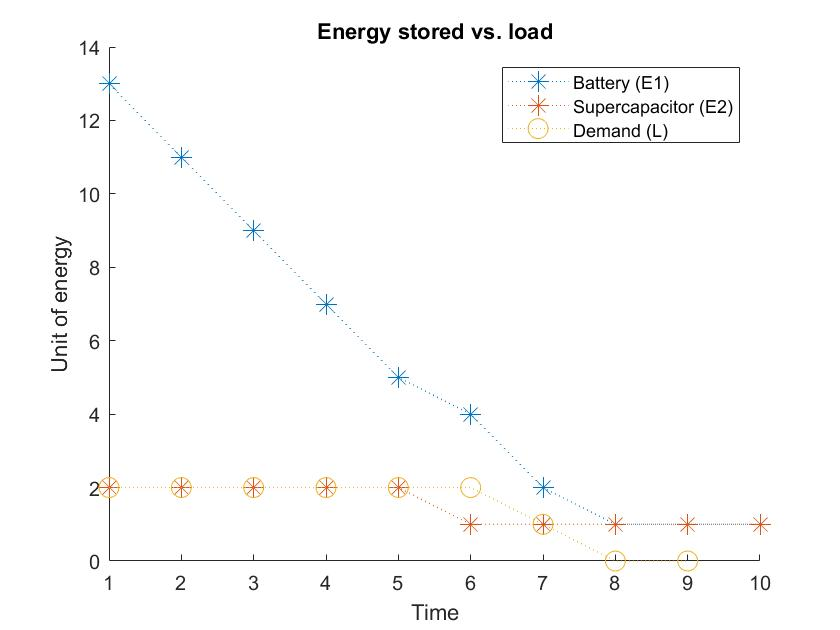
\includegraphics[scale=0.2]{EnergyStoredvsload_ConstantLoad(E1_max=13,E2_max=2).jpg}}
\caption{Testing optimal policy online with a constant demand sequence. Test size: N=$14\cdot3=42$, M=16.}
\label{fig:ConstDemand}
\end{figure}
\begin{figure}[htbp]
\centerline{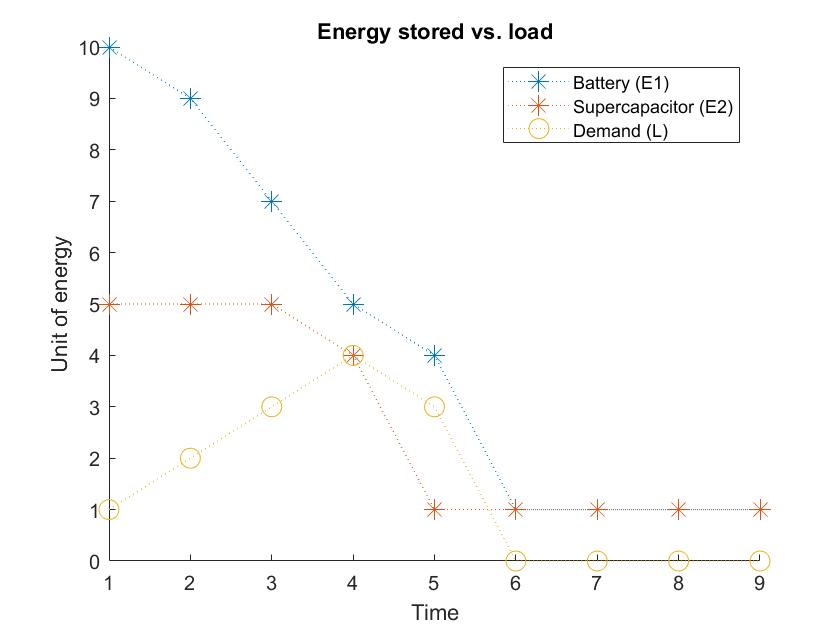
\includegraphics[scale=0.2]{EnergyStoredvsload_RampLoad(E1_max=10,E2_max=5).jpg}}
\caption{Testing optimal policy online with a ramp demand sequence. Test size: N=$11\cdot6=66$, M=16.}
\label{fig:RampDemand}
\end{figure} This result is expected because there is low cost for steady use of the battery (constant demand) or for limited cycling (ramp demand).

On the other hand, for fluctuating demand, the supercapacitor is used more, as illustrated in Figure \ref{fig:FluctuatingDemand}.
\begin{figure}[htbp]
\centerline{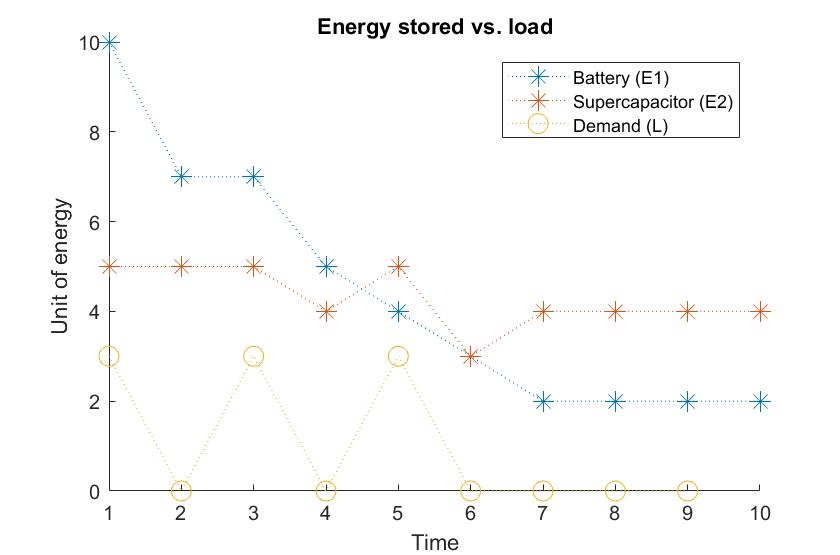
\includegraphics[scale=0.2]{EnergyStoredvsFluctuatingLoad(E1=10,E2=5).jpg}}
\caption{Testing optimal policy online with a fluctuating demand sequence. Test size: N=$11\cdot6=66$, M=16.}
\label{fig:FluctuatingDemand}
\end{figure} Clearly, the supercapacitor is now discharged at the start. However, this is still not as much use as expected. It was observed that by reducing the discharging efficiency of the battery, the supercapacitor is used more often (see Figure \ref{fig:FluctuatingDemand_LowBattEff}).
\begin{figure}[htbp]
\centerline{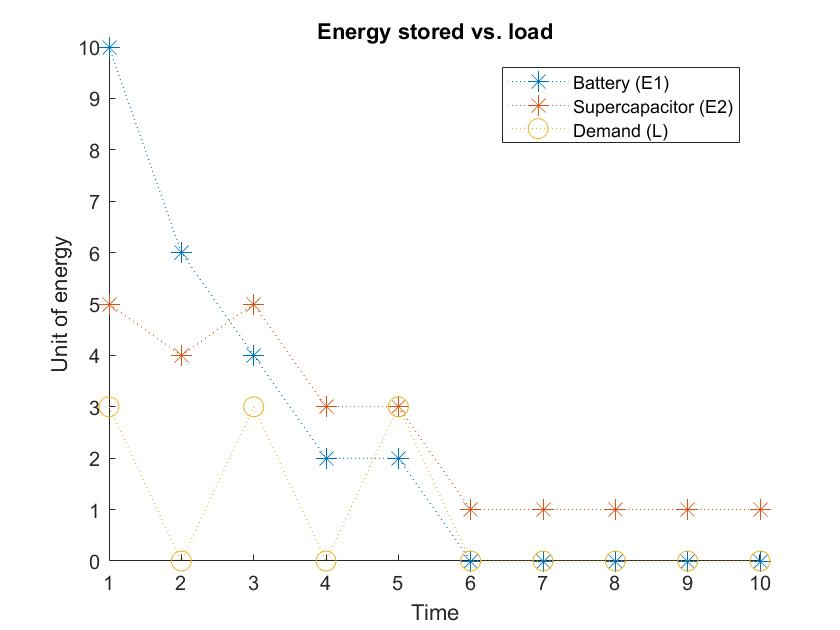
\includegraphics[scale=0.2]{EnergyStoredvsFluctuatingLoad_LowBattEff(E1=10,E2=5).jpg}}
\caption{Testing optimal policy online with a fluctuating demand sequence. Test size: N=$11\cdot6=66$, M=16. Lower battery efficiency (50\%).}
\label{fig:FluctuatingDemand_LowBattEff}
\end{figure} Hence, it is concluded that discharging the battery at the start of the sequence is still preferred because of the higher probability of large initial demands, unless the battery is inefficient.

One should also note how the battery is used to charge the supercapacitor, too. This can be seen, for example, in Figure 3 at time 4, where there is no demand but there are still exchanges in the energy between the storage devices. This also confirms that the optimal policy makes forecasts, since a trade-off is made between instantaneous transfer loss and satisfying fluctuating demands at a later time by preemptively charging the supercapacitor. Were it not for the benefits of the latter, there would be no reason for such energy exchanges.


%Finally, in addition to quantifying the error for LP, the LP is also compared to DP based on computational complexity. Table II provides simulation results for the number of iterations as the model size and tolerances (of \textit{both} programs) are varied.

%The experimental results in this table show that LP generally takes longer to converge for small problems, but is faster for large problems. Hence, this suggests that the LP formulation may be a more efficient program for this two-storage application.

%While the size of problems and number of cost evaluations were compared in Sections 4 and 6 for the general case, the number of iterations very application-dependent, as previously explained.

\section{Conclusion}
In conclusion, this paper has developed and optimized a model for energy transfers from two parallel storage devices satisfy a random demand. The model is an extension of the case with a single storage device, and was formulated using dynamic programming. Its optimal control policy can be applied to exactly satisfy a real-time demand, making it suitable for applications such as EVs.

Based on the timescales associated with this application, the DP was formulated as an infinite horizon problem. Most importantly, in order to resolve the curse of dimensionality, the solution was approximated by solving an approximate LP. To this end, the basis functions for the linear approximation were generated through a combination of state aggregation and monomials of state indices.

Lastly, the final program was simulated with three classes of demand to determine the optimal control in each case. As expected, it was found that high-energy or steady demands lead to more use of the battery, whereas fluctuating demand leads to more use of the complementary storage device. This means the policy produced by the program should work to reduce battery degradation, based on literature reviewed.

The final simulation results confirm that the approximate LP does allow for determining an optimal policy. Further work remains to be done to incorporate regenerative braking into this model.

\printbibliography

\end{document}